\subsubsection{\texttt{RF-8}: visualización de diferencias con solución}
\label{subsec:rf8}

Este requisito busca completar el objetivo del \texttt{RF-7.1} ---\referenciaSeccion{subsec:rf7}---, por el que se permite a los estudiantes descargar las soluciones de los ejercicios que dispongan de ella a partir de su publicación por parte del profesor.

El presente requerimiento aborda la creación de una característica que permita a los estudiantes visualizar gráficamente las diferencias que existan entre la propuesta de solución del profesor y su propia resolución del ejercicio. Para ejecutar esta funcionalidad, se han llevado a cabo las siguientes actuaciones:
\begin{itemize}
    \item Implementación de un algoritmo basado en el recorrido recursivo en profundidad de los directorios locales para obtener estructuras de datos arborescentes en memoria que reflejasen los contenidos de los directorios asociados tanto a la propuesta del propio alumno como a la solución descargada.
    \item Diseño y confección de un algoritmo que, dadas las dos estructuras arborescentes anteriormente detalladas, genera un nuevo árbol resultante de la combinación de los nodos de ambos árboles manteniendo en memoria el árbol de origen y preservando el orden alfabético de los nodos.
    \item Incorporación de los elementos de interacción con el usuario necesarios para que los estudiantes pudiesen visualizar la relación de ficheros existentes en el árbol obtenido mediante la ejecución de los dos algoritmos anteriores junto con su procedencia, incluyendo un cuadro de diálogo que muestra los ficheros y directorios del árbol resultante de la combinación y un botón habilitado tras descargar la solución que permite ejecutar la presente funcionalidad. En la \referenciaFigura{fig:reqf8-1} se capturan sendos elementos y señalan en color naranja y verde, respectivamente.
    \begin{itemize}
        \item En caso de que se seleccione un fichero únicamente existente en uno de los dos directorios, se abrirá en una nueva pestaña del entorno de desarrollo como un fichero simple.
        \item Por otro lado, en caso de que el fichero escogido exista en ambas procedencias, se mostrará un visor de diferencias entre ambos ficheros.
    \end{itemize}
\end{itemize}

\begin{figure}[ht]
    \centering
    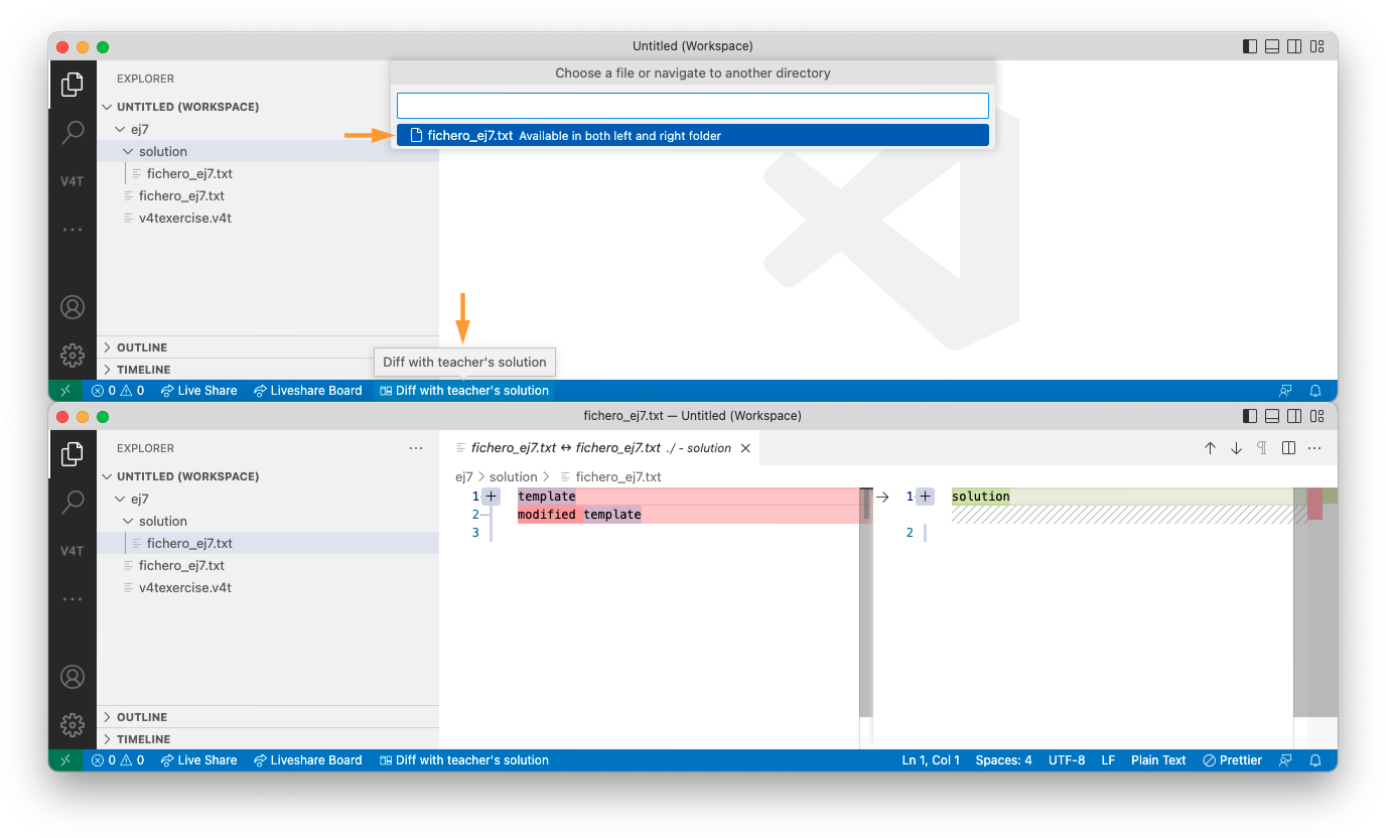
\includegraphics[width=\textwidth]{imagenes/utilizadas/4-3-implementacion/rf8-1.png}
    \caption{Captura de la extensión en la que se ejecuta la diferenciación entre la solución del docente y la propuesta del estudiante.}
    \label{fig:reqf8-1}
\end{figure}
